\documentclass[11pt]{article}

\input{../../preamble.tex}

\usepackage[margin=1in]{geometry}
\usepackage{amsmath,amssymb,bm}
\usepackage{graphicx}
\usepackage{float}
\usepackage{setspace}
\usepackage{tikz}
\usetikzlibrary{calc}

% ---------- Small helpers ----------
\newcommand{\kb}[1]{\bm{k}_{#1}}
\newcommand{\ob}[1]{\bm{o}_{#1}}
\newcommand{\vb}{\bm{v}}
\newcommand{\wb}{\bm{\omega}}
\newcommand{\J}{\bm{J}}
\newcommand{\q}{\bm{q}}
\newcommand{\qd}{\dot{\bm{q}}}
\newcommand{\twist}{\begin{bmatrix}\vb\\ \wb\end{bmatrix}}

\begin{document}

\begin{center}

{\Large University of British Columbia}

\vspace{0.2cm}

MECH 464/563 EECE 442/589: Introduction to Robotics

\vspace{0.2cm}

{\large Assignment \#5, due Friday March 6}

\end{center}

\vspace{0.5cm}

\noindent
\textbf{Exercise \#1. (50 points)}

\vspace{0.3cm}

Consider the Gen 3 Kinova 6DOF robot shown here. We do not follow the “DH Table”
from the User’s Guide (uploaded), as it does not follow the DH convention
and has mistakes in it. From the schematic diagram, and keeping the sign and
directions of the axes as in the User’s Guide, we can derive the following DH Table,
where $
l_0 = 0.1564 + 0.1284,
l_2 = 0.410,
l_3 = 0.0064 - 0.0054,
l_4 = 0.2083 + 0.1059,
l_6 = 0.1059 + 0.0615.
$
\begin{center}
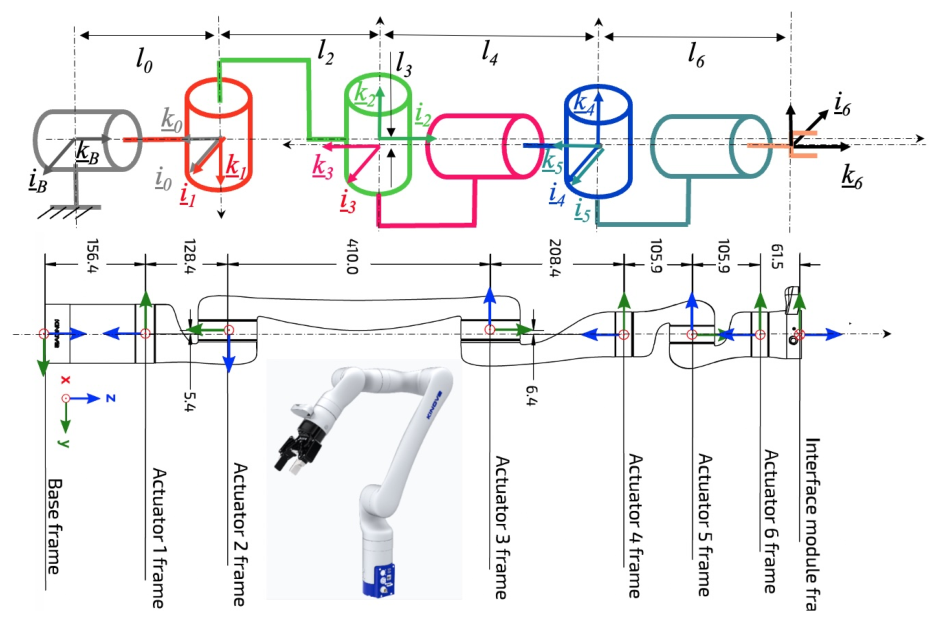
\includegraphics[width=0.9\textwidth]{kinova_robot.png}
\end{center}

\vspace{0.3cm}

\begin{center}
\textbf{Table 1: Kinova Gen3 Classical DH parameters with joint limits}
\end{center}

\begin{center}
\begin{tabular}{c c c c c c}
$i$ & $\theta_i$ (rad) & $d_i$ (m) & $a_i$ (m) & $\alpha_i$ (rad) & Joint limits (deg) \\
\hline
0 (from base) & 0.0 & $l_0$ & 0.0 & $\pi$ & -- \\
1 & $(q_1)$ & 0.0 & 0.0 & $\pi/2$ & $(-\infty,+\infty)$ \\
2 & $(q_2)-\pi/2$ & 0.0 & $l_2$ & $\pi$ & $[-128.9^\circ,128.9^\circ]$ \\
3 & $(q_3)-\pi/2$ & $-l_3$ & 0.0 & $-\pi/2$ & $[-147.8^\circ,147.8^\circ]$ \\
4 & $(q_4)$ & $-l_4$ & 0.0 & $-\pi/2$ & $(-\infty,+\infty)$ \\
5 & $(q_5)$ & 0.0 & 0.0 & $\pi/2$ & $[-120.3^\circ,120.3^\circ]$ \\
6 (to interface) & $(q_6)+\pi$ & $-l_6$ & 0.0 & $\pi$ & $(-\infty,+\infty)$
\end{tabular}
\end{center}

\vspace{0.5cm}

\noindent
(a) Write a MATLAB function to find the forward kinematics homogeneous matrix
$^{B}T_{6}(q)$ from the DH table, giving coords of $\{\tilde{o}_6, C_6\}$ in
$\{\tilde{o}_B, C_B\}$.

\vspace{0.3cm}

\noindent
(b) Find the manipulator geometric Jacobian. In which robot configuration is the
robot Jacobian singular?


\vspace{0.3cm}

\textbf{Solution.}

Every joint is spherical, so we have a manipulator jacobian of the form:

\[
J =
\begin{bmatrix}
k_0 \times (\tilde{o}_6 - \tilde{o}_0) &
k_1 \times (\tilde{o}_6 - \tilde{o}_1) &
k_2 \times (\tilde{o}_6 - \tilde{o}_2) &
k_3 \times (\tilde{o}_6 - \tilde{o}_3) &
k_4 \times (\tilde{o}_6 - \tilde{o}_4) &
k_5 \times (\tilde{o}_6 - \tilde{o}_5) \\
k_0 & k_1 & k_2 & k_3 & k_4 & k_5
\end{bmatrix}.
\]

Since joints 4, 5, and 6 form a spherical wrist, the origins $\tilde{o}_3$, $\tilde{o}_4$, and $\tilde{o}_5$ may be taken to coincide for the purpose of the Jacobian calculation. In particular, we use $\tilde{o}_3 = \tilde{o}_4 = \tilde{o}_5$.
Also, from the geometry of the manipulator, the axes $k_1$ and $k_2$ are antiparallel, so that $k_2 = -k_1$, 
and the first two frame origins coincide: $\tilde{o}_0 = \tilde{o}_1.$

Using these observations, the geometric Jacobian can be written in the equivalent form
\[
J \sim_{\mathrm{eq}}
\begin{bmatrix}
k_0 \times (\tilde{o}_6 - \tilde{o}_0) &
k_1 \times (\tilde{o}_6 - \tilde{o}_0) &
-k_1 \times (\tilde{o}_6 - \tilde{o}_2) &
k_3 \times (\tilde{o}_6 - \tilde{o}_3) &
k_4 \times (\tilde{o}_6 - \tilde{o}_3) &
k_5 \times (\tilde{o}_6 - \tilde{o}_3) \\
k_0 & k_1 & -k_1 & k_3 & k_4 & k_5
\end{bmatrix}.
\]

Now add to the first block row the second block row multiplied by $(\tilde{o}_6-\tilde{o}_3)$.
Then, $J$ is singular if and only if the following matrix is singular:
\[
\widehat{J} \sim_{\mathrm{sing}}
\begin{bmatrix}
k_0 \times (\tilde{o}_3 - \tilde{o}_0) &
k_1 \times (\tilde{o}_3 - \tilde{o}_0) &
-k_1 \times (\tilde{o}_3 - \tilde{o}_2) &
0 &
0 &
0 \\
k_0 & k_1 & -k_1 & k_3 & k_4 & k_5
\end{bmatrix}.
\]

This is singular iff at least two of the column vectors are linearly dependent.
We analyze the robot to see when this can be the case.
First, though $k_4$ will always be perpendicular to $k_3$ and $k_5$, in the case of wrist gimbal lock we can have $k_3  \parallel k_5$.

Now, since $\tilde{o}_3$ is offset from $k_0$, it can never be the case that $\tilde{o}_{3} - \tilde{o}_{2} \parallel \tilde{o}_{3} - \tilde{o}_{0}$, $k_1 \parallel (\tilde{o}_6 - \tilde{o}_0)$ or $k_1 \parallel (\tilde{o}_6 - \tilde{o}_2)$, or $k_0 \parallel (\tilde{o}_3 - \tilde{o}_0)$, so we have no singularities arising from the first 3 joints.

Therefore, the only singularity happens when $k_3 \parallel k_5$.

\vspace{0.3cm}

\noindent
(c) Write a MATLAB function to compute the robot Jacobian for a given set of
joint angles. For example, in response to a function call or to user input, e.g.,

\[
q =
\begin{bmatrix}
45^\circ & -45^\circ & 45^\circ & 0^\circ & -30^\circ & 90^\circ
\end{bmatrix},
\]

the program will output the manipulator Jacobian, as a $6\times6$ matrix of
coordinates relative to the base coordinate system $\{\tilde{o}_B, C_B\}$,
relating joint velocities to end-effector velocities in base frame.

Use your code to compute the manipulator Jacobian and its condition number for a
number of interesting sets of joint configurations, including

\[
q =
\begin{bmatrix}
0^\circ & 90^\circ & 90^\circ & 0^\circ & 90^\circ & 0^\circ
\end{bmatrix}^T,
\]

\[
q =
\begin{bmatrix}
0^\circ & 90^\circ & 90^\circ & 0^\circ & 0^\circ & 0^\circ
\end{bmatrix}^T,
\]

\[
q =
\begin{bmatrix}
0^\circ & 7.2767^\circ & 15^\circ & 0^\circ & 90^\circ & 0^\circ
\end{bmatrix}^T,
\]

and comment on the results.

\vspace{0.3cm}

\noindent
Note: It may be useful to render the Kinova using the Robotics Toolbox by Peter
Corke.

\vspace{0.5cm}

\noindent
\textbf{Exercise \#2. (50 points)}

\vspace{0.3cm}

Write four Matlab functions that solve the respective Kahan problems. The returned
angles should be in degrees. Include the proper number of solutions or return
NaN (not a number) for an invalid solution. Apply a reasonable tolerance
threshold when determining if a solution exists.

\vspace{0.3cm}

\[
\theta = \text{KahanP1}(s,t)
\]

finds the angle between $s$ and $t$ ($\theta \in [0,180^\circ]$).

\vspace{0.3cm}

\[
\theta = \text{KahanP2}(\hat{s},u,v)
\]

solves

\[
e^{\theta \hat{s}\times} u = v
\]

for $\theta \in (-180^\circ,180^\circ]$.

\vspace{0.3cm}

\[
[\phi,\theta] = \text{KahanP3}(\hat{s},\hat{t},u,\hat{v})
\]

solves

\[
e^{\theta \hat{s}\times}u = e^{\phi \hat{t}\times}v
\]

with $(\theta,\phi \in (-180^\circ,180^\circ])$.

\vspace{0.3cm}

\[
\theta = \text{KahanP4}(a,b,c)
\]

finds the supplementary angle formed by sides $a$ and $b$ of triangle $abc$
($\theta \in [0,180^\circ]$).

\vspace{0.5cm}

\noindent
\textbf{Exercise \#3: (50 points)}

\vspace{0.3cm}

(a) Solve the inverse kinematics of the Kinova 6DOF manipulator.

\vspace{0.3cm}

(b) Write a MATLAB program that provides all inverse kinematics solutions.
Inputs are the coordinates in base frame of the desired end-effector location
($\tilde{o}_d$), approach vector ($k_d$) and sliding vector ($j_d$).

Output all valid sets of joint angles (in degrees) that achieve this.

Verify that your program works for several distinct sets of inputs, including
the joint variables listed under Problem 1(c), by feeding each of your
solutions into the forward kinematics (briefly explain how you chose the inputs).

Document your code with references to your inverse kinematics solution.
Carefully consider how many possible solutions there are, considering the
joint ranges in the table provided.

\vspace{0.4cm}

\noindent
Hint: Since $\tilde{o}_4$ is the centre of the wrist, we have

\[
\tilde{o}_4 - \tilde{o}_0 =
e^{-\theta_1 k_B \times}
e^{\theta_2 j_B \times}
\left[
l_2 k_B
+
e^{-\theta_3 j_B \times}
(l_4 k_B + l_3 j_B)
\right]
\]

\[
=
e^{-\theta_1 k_B \times}
e^{\theta_2 j_B \times}
\left[
l_2 k_B + l_3 j_B
+
e^{-\theta_3 j_B \times} l_4 k_B
\right]
\]

where we moved $l_3 j_B$ outside the rotation $e^{-\theta_3 j_B\times}$ since
$l_3 j_B$ is aligned with the rotation axis.

Projecting on the plane $k_B - i_B$ we have Kahan’s problem P4.
Solve for $\theta_3$, then we are left with Kahan’s problem P3.

\vspace{3em}

\textbf{Solution.}
(a)
We follow the hint, and start with:
\[
    \tilde{o}_{4} - \tilde{o}_0 = e^{-\theta_1 k_B \times } e^{\theta_2 j_B \times} \left[ l_2 k_B + e^{-\theta_3 j_B \times } (l_4 k_B + l_3 j_B) \right] 
.\]
Premultiplying by $e^{-\theta_2 j_B \times}e^{\theta_1 k_B \times}$, we have
\begin{align}
    e^{-\theta_2 j_B \times}e^{\theta_1 k_B \times} (\tilde{o}_{4} - \tilde{o}_0) &= l_2 k_B + e^{- \theta_3 j_B \times } (l_4 k_B + l_3 j_B) \label{eq:label_name}
.\end{align}
However, $j_B$ doesn't rotate about $j_B$, so we have
\begin{align*}
    e^{-\theta_2 j_B \times}e^{\theta_1 k_B \times} (\tilde{o}_{4} - \tilde{o}_0) &= l_2 k_B + l_3 j_B + e^{- \theta_3 j_B \times } l_4 k_B
.\end{align*}
Next, we subtract $l_3 j_B$ from both sides.

\begin{align*}
e^{-\theta_2 j_B \times}e^{\theta_1 k_B \times} (\tilde{o}_{4} - \tilde{o}_0) - l_3 j_B &= l_2 k_B + e^{- \theta_3 j_B \times } l_4 k_B
.\end{align*}
The vector on the right is purely in the $k_B$-$i_B$ plane, so we can apply pythagorus to solve the length of the quantity on the left:
\[
\|e^{-\theta_2 j_B \times}e^{\theta_1 k_B \times} (\tilde{o}_{4} - \tilde{o}_0) - l_3 j_B \|^2 = \|\tilde{o}_4 - \tilde{o}_0\|^2 - l_3^2
.\] 
Thus, we have a triangle with sidelengths $l_2$, $l_4$, and $\sqrt{\|\tilde{o}_4 - \tilde{o}_0\|^2 - l_3^2}$, with the triangle then has an exterial angle $\theta_3$ outside the sidelengths $l_2$ and $l_4$.

\begin{center}

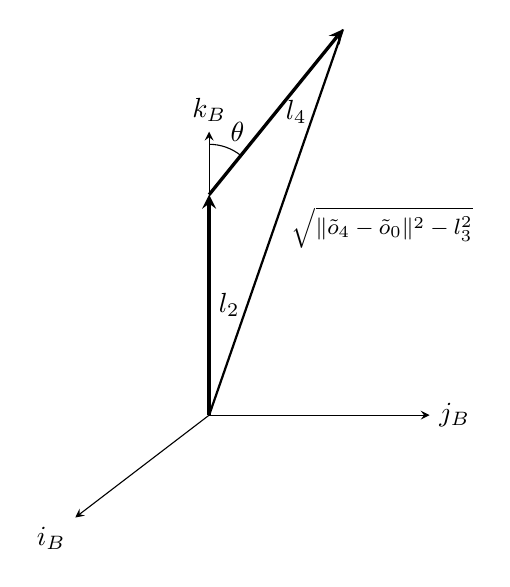
\begin{tikzpicture}[scale=2.0, >=stealth]

% Points
\coordinate (O) at (0,0);
\coordinate (A) at (0,1.4);
\coordinate (B) at (0.85,2.45);

% Base frame
\draw[->] (O) -- (1.4,0) node[right] {$j_B$};
\draw[->] (O) -- (-0.85,-0.65) node[below left] {$i_B$};
\draw[->] (O) -- (0,1.8) node[above] {$k_B$};

% First link
\draw[very thick,->] (O) -- (A);
\node[right] at ($(O)!0.5!(A)$) {$l_2$};

% Second link
\draw[very thick,->] (A) -- (B);
\node[right] at ($(A)!0.5!(B)$) {$l_4$};

% Diagonal
\draw[thick] (O) -- (B);

% Diagonal label
\node[font=\footnotesize, sloped, above] at (1.1, 1)
    {$\sqrt{\|\tilde{o}_{4} - \tilde{o}_{0}\|^2 - l_{3}^2}$};

% Angle theta
\draw (A) ++(0,0.32) arc[start angle=90,end angle=51,radius=0.32];
\node at (0.18,1.8) {$\theta$};

\end{tikzpicture}

\end{center}

This is a KP4 problem, which we then solve for $\theta_3$.
For reference in the computer program, I will write this out explicitly:
\begin{equation}
    |\theta_3| = KP_4(l_2, l_4, \sqrt{\|\tilde{o}_4 - \tilde{o}_0\|^2 - l_3^2}
)
\end{equation}


With $\theta_3$, we can then compute two possible solutions $w_{\pm} = l_2 k_B + l_3j_B + e^{\mp \theta_3 j_B \times } (l_4 k_B + l_3 j_B)$.
Then, equation \eqref{eq:label_name} gives us
\begin{align*}
    e^{-\theta_2 j_B \times}e^{\theta_1 k_B \times} (\tilde{o}_{4} - \tilde{o}_0) &= w_{\pm}\\
   e^{\theta_1 k_B \times} (\tilde{o}_{4} - \tilde{o}_0) &= e^{\theta_2 j_B \times }w_{\pm}
.\end{align*}
This is a KP3 problem.
For each vector $w_{\pm}$ we can solve for potentially 2 solutions that are pairs $(\theta_1, \theta_2)$.

The $KP_{3}$ problem is stated here:
\begin{align}
    u &= \tilde{o}_4 - \tilde{o}_0\\
    w_{\pm} &= l_2 k_B + l_3j_B + e^{\mp \theta_3 j_B \times }l_4 k_B  \\
    (\theta_1, \theta_2)_i &= KP_{3} (u, w_{\pm}, k_B, j_B) 
.\end{align}
Since the range of $\theta_2$ is limited, these solutions must be tested to ensure that they obey the constraints.

Now, having solved for potential values $\theta_1, \theta_2, \theta_3$, we fix a potential solution, and then use forward kinematics to compute $C_3, o_3$ in the frame $C_B, o_B$.
Following the notes, we have that $C_6$ can be obtained from $C_3$ following a series of rotations:

\begin{align*}
    \underline{C}_6 &= \underline{C}_3 e^{\theta_4 k \times } e^{\theta_5 j \times } e^{\theta_6 k \times}
.\end{align*}

Next, we re-arrange, and consider the vector $j$ in each co-ordinate frame (which we are given, since this is the second column of $\underline{C}_6$ and $\underline{C}_3$) respectively:

\begin{align*}
    \underline{C}_6 e^{-\theta_6 k \times } &= \underline{C}_3 e^{\theta_4 k \times } e^{\theta_5 j \times }\\
    e^{-\theta_6 \underline{k}_6 \times } \underline{C}_6 &= e^{\theta_4 \underline{k}_3 \times }  \underline{C}_3 e^{\theta_5 j \times }\\
    e^{-\theta_6 \underline{k}_6 \times } \underline{C}_6 j &= e^{\theta_4 \underline{k}_3 \times }  \underline{C}_3 e^{\theta_5 j \times }j\\
    e^{-\theta_6 \underline{k}_6 \times } \underline{C}_6 j &= e^{\theta_4 \underline{k}_3 \times }  \underline{C}_3 j\\
    e^{-\theta_6 \underline{k}_6 \times } \underline{j}_6 &= e^{\theta_4 \underline{k}_3 \times }  \underline{j}_3
.\end{align*}

This is a $KP_3$ problem, which we can solve for $\theta_4$, and $\theta_6$ candidates.
That is:
\[
\theta_4, -I \theta_6 = KP_{3}(k_6,j_6,k_3,j_3)
.\]

Knowing $\theta_4$, we use forward kinematics to solve for $\underline{C}_4 = \underline{C}_3e^{\theta_4 k \times }$, and

\begin{align*}
    \underline{C}_6 e^{-\theta_6 k\times } &= \underline{C}_4 e^{\theta_5 j\times }\\
    \underline{C}_6 e^{-\theta_6 k\times } k &= \underline{C}_4 e^{\theta_{5} j \times } k \\
    k_6 &= e^{\theta_5 \underline{j}_4 \times } k_4
.\end{align*}

Since we have $C_4$, we know $j_4$, $k_4$, and since we have $C_6$, we know $k_6$.
This is a $KP_2$ problem, so we have

\begin{align}
\theta_5 &= KP_2 (\underline{j}_4,\underline{k}_4,\underline{k}_6)
.\end{align}

With this process, we can then compute a list of possible candidates for $\vec{\theta} = (\theta_1, \theta_2, \theta_3, \theta_4, \theta_5, \theta_6)$.
\end{document}
